\section{Diagrama de Packages}
De forma a organizarmos melhor a aplicação, dividimos o sistema geral em quatro subsistemas: o Facade (que corresponde à ConfiguraFácil), o gContas, o gConfig e o gFabrica. Como tal, construímos o seguinte diagrama de pacotes:
\begin{center}
 	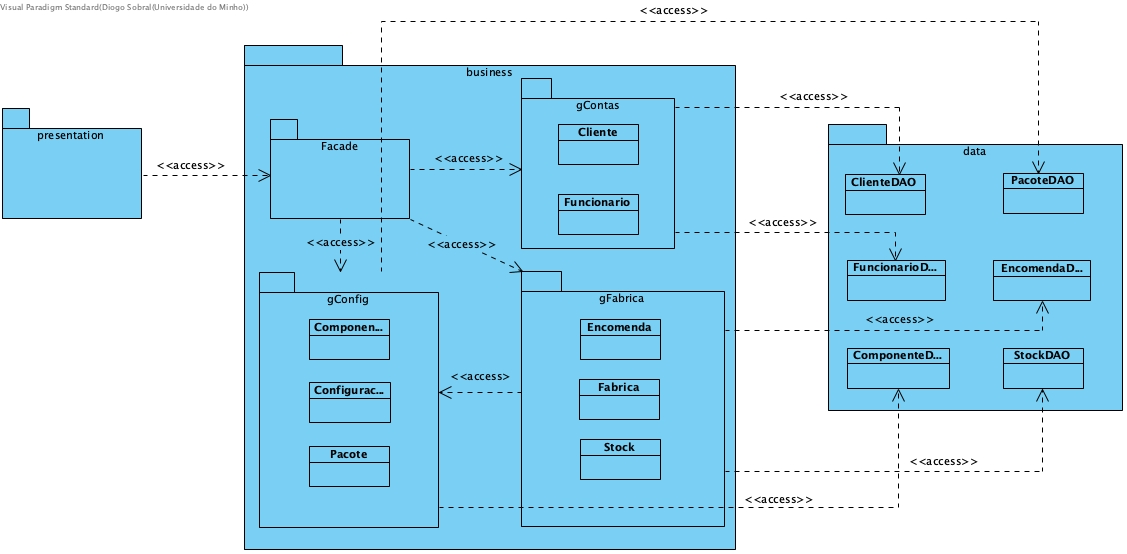
\includegraphics[width=6in]{VPP/Packages.jpg}
\end{center}
\newpage
\subsection{Camada de Negócio - Subsistemas}
\begin{itemize}
    \item \textbf{ConfiguraFácil(Facade)}\newline
    O ConfiguraFácil será responsável por produzir a ligação entre a interface gráfica e camada de negócio.
    \item \textbf{gContas} \newline
    A aplicação do stand terá de guardar e tratar informação relativa aos seus utilizadores e clientes. O gContas será o subsistema responsável por garantir que tudo isto é possível.
    \item \textbf{gConfig} \newline
    O objetivo principal da aplicação é conseguir configurar e realizar pedidos específicos por parte dos clientes. O gConfig será responsável por permitir a realização de configurações sem que estas se tornem inviáveis.
    \item \textbf{gFabrica} \newline
    A aplicação também terá capaz de gerir a produção de encomendas e garantir a existência de stock da sua fábrica. Assim, o gFabrica fica responsável pela gerência das encomendas do cliente e por gerir o stock disponível.
\end{itemize}
